\documentclass[letterpaper,11pt,twocolumn]{article}
\usepackage[utf8]{inputenc}
\usepackage[T1]{fontenc}
\usepackage[letterpaper,margin=0.55in]{geometry}
\usepackage{tgbonum}
\usepackage{csquotes}
\usepackage{enumitem}
\usepackage{parskip}
\usepackage{titlesec}
\usepackage{fancyhdr}
\usepackage{tabularx}
\usepackage{booktabs}
\usepackage{multirow}
\usepackage{tikz}
\usetikzlibrary{arrows.meta,positioning,shapes.geometric}
\usepackage[dvipsnames]{xcolor}
\usepackage[hidelinks]{hyperref}

\DeclareTextFontCommand{\textbfit}{\bfseries\itshape}
\newcommand{\Imperium}{\textit{Imperium}}
\newcommand{\SpaceEmpires}{\textit{Space Empires: 4X}}
\newcommand{\CloseEncounters}{\textit{Close Encounters}}
\newcommand{\RU}{RU}

\title{%
  Space Empires: Imperium \\
  \vspace{0.4em}
  \large A two-player Traveller-era campaign game}
\author{Designed by Daniel J. Berger}
\date{Version 0.1 --- Playtest Draft}

\setlength{\columnsep}{2em}
\setcounter{secnumdepth}{3}
\setcounter{tocdepth}{2}
\setlist{nosep,leftmargin=*}
\raggedbottom

\pagestyle{fancy}
\fancyhead{}
\fancyfoot{}
\fancyhead[L]{\small Space Empires: Imperium v0.1}
\fancyfoot[R]{Page \thepage}
\renewcommand{\headrulewidth}{0.2pt}

\titlespacing{\section}{0pt}{1.25em}{0.5em}
\titlespacing{\subsection}{0pt}{1em}{0.35em}
\titlespacing{\subsubsection}{0pt}{0.8em}{0.25em}

\titleformat{\section}
  {\Large\bfseries}
  {[\thesection.0]}
  {0.5em}
  {}
\titleformat{\subsection}
  {\large\bfseries}
  {[\thesubsection]}
  {0.5em}
  {}
\titleformat{\subsubsection}
  {\normalsize\bfseries}
  {[\thesubsubsection]}
  {0.5em}
  {}

\begin{document}
  \maketitle
  \onecolumn
  \tableofcontents
  \vfill
  \begin{center}
    \small
    This is a non-commercial fan design. Traveller, \Imperium,
    \SpaceEmpires, and \CloseEncounters\ remain the property of their
    respective rights holders. This document is not endorsed by GDW, GMT
    Games, or the current Traveller rights holders.
  \end{center}
  \clearpage
  \twocolumn

  \section{INTRODUCTION}

In 2113 the expanding Terran Confederation reaches the edge of the Ziru
Sirka, the First Imperium. Neither polity can accept the other's idea of
order. What begins as a frontier dispute becomes a succession of short,
violent wars separated by uneasy peaces. Terra learns quickly; the Imperial
provincial governor commands greater resources but must answer to a distant
Emperor.

\textit{Space Empires: Imperium} is a two-player strategic campaign. It keeps
the point-to-point jump map, political asymmetry, Glory system, and repeated
wars of GDW's \Imperium. It uses the ship groups, firing classes, attack and
defense values, hull damage, screening, fighters, and ground forces from
\SpaceEmpires\ and \CloseEncounters. Its Ship Yards make the primary Worlds
the vulnerable industrial centers of each side. A shared card deck introduces
a small amount of operational surprise.

Fleet combat specifically reconciles the two parent systems rather than
discarding either one. Fleets contest Long or Close Range and choose beam,
missile, or mixed armament in the manner of \Imperium, while attacks use the
printed classes, d10 Hit Numbers, screening, and hull damage of
\SpaceEmpires. Traveller-inspired pickets, point defense, and sandcasters
make the range and weapon choices visible at fleet scale.

This is an alpha playtest design. Its systems are complete enough to play the
\textit{First Shots} war, but the force mix and economy have not yet been
balanced through repeated play.

\subsection{The Central Design Choice}

The game is not a full 4X game. The map is known, the frontier is already
settled, and there are no non-player aliens. Players fight over an existing
political geography. Technology changes slowly and only between wars. The
interesting decisions should be where to build a logistics chain, whether to
hold missile range or close to beam range, when to commit the fleet, whether
to risk an invasion before orbital combat is settled, and how much political
capital to spend for a short-term advantage.

\subsection{Rules Hierarchy}

Use these rules first. If they do not address a situation, use the following
sources in order:

\begin{enumerate}
  \item this rulebook and the text in its card manifest;
  \item \SpaceEmpires\ rules for ships, groups, damage, screening, fighters,
    and retreat;
  \item \CloseEncounters\ section 14 for transports and ground combat; and
  \item \Imperium\ only for interpretation of its map and named systems.
\end{enumerate}

Rules from a parent game that concern hex movement, exploration, colony
growth, aliens, or that game's sequence of play do not apply. When printed
card text disagrees with the manifest in this rulebook, the manifest controls.

\subsection{Rounding and Dice}

Round fractions down unless a rule says otherwise. A ``die'' or ``d10'' is a
ten-sided die; a zero face counts as 10. ``2d6'' means two six-sided dice
added together.

  \section{GAME PARTS}

\subsection{Required Material}

You need the map and charts from \Imperium; ship, group, numeral, technology,
damage, colony, Base, Ship Yard, and resource markers from \SpaceEmpires; and
Transport and Ground Unit counters from \CloseEncounters. You also need the
42-card Imperium Deck in the \texttt{Cards} directory, two d6, several d10,
and spare markers for missile depletion and defensive reactions.
Each player should also have one copy of the separate landscape Logistics \&
Fleet Record aid. Keep its Fleet Group Manifest hidden from the opponent.

The original \Imperium\ ship and troop counters are not used. Its World and
Outpost counters may be used if they are easier to read than the substitutions
below.

\subsection{Map Terms}

A \textbf{system} is a named stellar hex and every planetary surface box
attached to it. A green line joining two stellar hexes is a \textbf{jump
route}; the joined systems are \textbf{adjacent}. Ordinary map hexes and
sublight movement are ignored.

A \textbf{primary surface} is a white planetary surface box. A \textbf{secondary
surface} is a red box. A binary system can contain two surfaces with different
owners. Space control is determined once for the whole stellar hex, while
surface control is determined separately for each box.

\subsection{Counter Substitutions}

\begin{tabularx}{\columnwidth}{@{}lX@{}}
\toprule
Game term & Counter used \\
\midrule
World & 5 Colony marker; use a Home marker at Sol and Gashidda \\
Outpost & 1 Colony marker \\
Neutralized & 3 Colony or spare status marker on a World \\
Planetary Defense & Base \\
Fleet Train & MS Pipeline \\
Resource Units & CP markers and track \\
\bottomrule
\end{tabularx}

Worlds and Outposts do not grow like \SpaceEmpires\ colonies. The number on
their substitute counter is only a reminder of their defensive Militia value.

\subsection{Units in Use}

The initial design uses Scouts (SC), Destroyers (DD), Cruisers (CA),
Battlecruisers (BC), Battleships (BB), Dreadnoughts (DN), Carriers (CV),
Fighters (F), Bases, Ship Yards (SY), Transports (TR), and the Ground Units
described in these rules. Their printed class, attack, defense, and hull values
are unchanged.

Colony Ships, Miners, Raiders, Mines, Minesweepers, Titans, alien ships, and
non-player forces are not used. The Minefield card does not require a Mine
counter.

\subsection{Groups and Stacks}

Use \SpaceEmpires\ group and numeral rules. A \textbf{group} contains one ship
type with identical technology and, where applicable, one Armament Package. A
\textbf{stack} is every friendly group that
moves together from one system. Ground Units and Fighters being carried move
with their Transport or Carrier but do not count as separate groups.

Groups stay face down on the map. Reveal them when required by combat or an
event, then conceal surviving groups after all combat in that system ends.

\subsection{Resource Units}

Resource Units (RU) replace Colony Points. One RU equals one CP for every
printed \SpaceEmpires\ cost. RU may be saved without limit between turns and,
in a campaign, between wars.

  \section{GENERAL SETUP}

\begin{enumerate}
  \item Choose a scenario and sides. Terra uses one \SpaceEmpires\ color and
    the Imperium another.
  \item Lay out the \Imperium\ map. Place Worlds, Outposts, Bases, fleets, and
    Ground Units listed by the scenario. Put Ground Units and Bases in their
    surface box; all other starting units begin in the stellar hex.
  \item Record each side's starting technology and capital-construction level,
    and record an Armament Package for every eligible ship group. Technology
    applies to every eligible friendly group.
  \item Put the Terran Turn marker at 0, the Imperial Turn marker at 11, and
    the Glory marker at 5. Put the Game Turn marker at 1.
  \item Put each RU marker at the scenario's starting amount. The first
    scenario begins with 0 RU.
  \item Shuffle the Imperium Deck. Deal the starting hands specified in
    section 12.
  \item Place purchased-unit counters, damage markers, d10s, and spare status
    markers near the map.
  \item The scenario identifies the First Player. The other side is the Second
    Player for the whole war.
\end{enumerate}

Starting ships require maintenance on Game Turn 1. No starting force may be
placed at a neutralized World or an unconnected Outpost unless the scenario
explicitly says otherwise.

  \section{SEQUENCE OF PLAY}

A war lasts no more than five Game Turns. Each Game Turn contains one joint
Logistics Phase followed by a Player Turn for each side. The First Player
always takes the first Player Turn.

\subsection{Game Turn Sequence}

\begin{enumerate}[label=\Alph*.]
  \item \textbf{Advance the clocks.} Move the Terran Turn marker up one space
    and the Imperial Turn marker down one space. Do this at the start of Game
    Turn 1 as well.
  \item \textbf{Joint Logistics Phase.} Both sides complete these steps, First
    Player first when order matters:
    \begin{enumerate}[label=\arabic*.]
      \item Political Events
      \item Determine Connections and Collect Income
      \item Pay Maintenance
      \item Draw, Discard, and Purchase Cards
      \item Receive Completed Production
      \item Purchase New Production
    \end{enumerate}
  \item \textbf{First Player Turn.}
    \begin{enumerate}[label=\arabic*.]
      \item First Movement Phase
      \item First Combat Phase
      \item Enemy Reaction Movement Phase
      \item Enemy Reaction Combat Phase
      \item Second Movement Phase
      \item Second Combat Phase
    \end{enumerate}
  \item \textbf{Second Player Turn.} Repeat the six steps above with the roles
    reversed.
  \item \textbf{End Phase.}
    \begin{enumerate}[label=\arabic*.]
      \item Remove temporary markers and restore temporary Militia.
      \item Check whether unsupported neutralized Worlds recover.
      \item Apply delayed Glory changes and check for the end of the war.
    \end{enumerate}
\end{enumerate}

\subsection{Phasing Player}

The player whose Movement or Combat Phase is in progress is the \textbf{Phasing
Player}. The opponent is the \textbf{Non-Phasing Player}. In a Reaction Phase,
the reacting player becomes the Phasing Player for that phase only.

\subsection{Combat Phase Order}

The Phasing Player chooses the order of contested systems. Completely resolve
one system before beginning another. In each system:

\begin{enumerate}
  \item resolve space combat, including any troop landings;
  \item resolve bombardment, if permitted;
  \item make final landings; and
  \item resolve every ground combat on a surface in that system.
\end{enumerate}

Combat is mandatory wherever opposing combat-capable ships occupy the same
stellar hex. Ground combat is mandatory wherever opposing Ground Units occupy
the same surface.

\subsection{First Player in Later Wars}

In the first war Terra is the First Player. In every later war, the loser of
the previous war is the First Player. The winner therefore deploys second but
moves second, reflecting the loser's preparations for renewed hostilities.

  \section{MOVEMENT AND LOGISTICS}

Ships move only by jumping along printed jump routes. A jump is movement from
one stellar hex directly to an adjacent stellar hex. The intervening map hexes
are never entered. Movement is voluntary, and groups may split or combine as
allowed by the \SpaceEmpires\ group rules.

\subsection{Refuelling}

A stack may make any number of jumps in a normal Movement Phase, but after it
enters a system it must refuel before it can leave that system in the same
phase. A stack can refuel at:

\begin{itemize}
  \item a friendly World or Outpost that is not neutralized;
  \item a friendly Fleet Train that began the phase in that system and has not
    moved during the phase; or
  \item any system, if the moving stack consists entirely of Scouts.
\end{itemize}

A stack can therefore travel rapidly down a prepared chain and make one final
jump beyond it. It must then stop. A source may refuel any number of stacks.
Enemy control of the stellar hex prevents refuelling there, even if a friendly
surface remains below.

\subsection{Enemy-Occupied Systems}

A stack stops when it enters a system containing enemy combat-capable ships.
It must fight in the following Combat Phase. A stack entering a system with
only enemy non-combat ships destroys those ships immediately and may continue
if it can refuel. An enemy-controlled surface does not by itself stop movement.

\subsection{Supply Status}

Supply is checked during the Joint Logistics Phase and lasts for the Game
Turn. A ship is \textbf{supplied} if it is:

\begin{itemize}
  \item in a system containing a connected friendly World or Outpost;
  \item in a system containing a friendly Fleet Train; or
  \item one jump from either of those locations along a jump route not blocked
    by enemy ships.
\end{itemize}

An unsupplied ship costs one additional RU to maintain and may make at most one
jump in each Movement or Reaction Movement Phase. Scouts ignore the movement
penalty but not the maintenance surcharge. A ship that becomes supplied later
in the turn does not lose its unsupplied marker until the next Logistics Phase.

\subsection{Fleet Trains}

MS Pipeline counters are Fleet Trains. A Fleet Train is a non-combat ship with
its printed hull and defense, a production cost of 5 RU, no maintenance cost,
and a speed of one jump per Movement Phase. It may not react. It provides fuel
only if it did not move in the current phase, but it provides supply during the
Logistics Phase simply by being present.

Fleet Trains are automatically screened while friendly combat ships remain.
They are destroyed if caught alone. A Fleet Train may bridge an empty system
when tracing an economic connection.

\subsection{Fighters and Ground Units}

Fighters cannot jump. They may operate at a friendly World or Outpost or be
carried by Carriers under \SpaceEmpires\ section 11. A Carrier carries three
Fighter groups. Fighters may transfer between a base and Carrier when the
Carrier is in the same system.

Ground Units cannot jump. A Transport carries up to six Ground Units using
\CloseEncounters\ section 14. Loading or unloading at a friendly surface does
not use movement, but a particular Ground Unit may be loaded and unloaded only
once in a Movement Phase.

\subsection{Reaction Movement}

During a Reaction Movement Phase the reacting player may move one stack from
one system. The stack may make up to its side's Reaction Allowance (two jumps
for Terra and three for the Imperium at the start of the campaign), subject to
refuelling, supply, and enemy-occupied-system rules. It need not move toward the Phasing Player.
All groups in the chosen stack need not end together, but no additional group
may begin reaction movement.

Only ships that participated in Reaction Movement may attack in the following
Reaction Combat Phase. Friendly units already present in the battle system may
join their combat normally. Bases, Ship Yards, and Fighters may fight if the
reaction stack ends in their system, but they do not themselves react.

Cards and technology can increase the number of reacting stacks or jumps. A
reaction stack can never make more than six jumps.

\subsection{Retreat Movement}

Retreat is part of combat, not a Movement Phase. A retreating group moves to
one adjacent system free of enemy combat-capable ships. It need not refuel, but
it may not participate again during the current Player Turn. A group with no
legal destination cannot retreat.

  \section{ECONOMICS AND PRODUCTION}

\subsection{Connections}

A Terran World is connected if a path can be traced from it to Sol. An Imperial
World is connected if a path can be traced from it to Gashidda. Trace through
jump routes and systems containing a friendly World, friendly Outpost, or
friendly Fleet Train. The endpoints count, and directly adjacent friendly
sites connect without an intermediate counter.

Enemy combat-capable ships block a path through their stellar hex. A
neutralized site cannot carry a path. An Outpost is connected if it can trace
to any connected friendly World. Several isolated Worlds may form a local
network, but none of them is connected until the network reaches the capital.

Determine all connections before either player collects income; they do not
change for economic purposes later in the phase.

\subsection{Income}

\begin{tabularx}{\columnwidth}{@{}Xrr@{}}
\toprule
Source & Terra & Imperium \\
\midrule
Provincial budget & --- & 10 \\
Connected World & 8 & 3 \\
Unconnected World & 6 & 1 \\
Connected Outpost & 1 & 0 \\
Unconnected Outpost & 0 & 0 \\
\bottomrule
\end{tabularx}

Neutralized Worlds and contested or enemy-held Outposts produce nothing.
Income is added to saved RU. Temporary political and card effects are applied
after the normal total is known.

\subsection{Maintenance}

Pay maintenance for every ship already on the map. The cost of one ship is its
printed Hull Size in RU, as in \SpaceEmpires. Fighters pay maintenance;
Fleet Trains, Bases, and Ground Units do not. A Carrier and its Fighters are
maintained separately. Each unsupplied ship costs one additional RU.

The owner chooses the order of payment. Any ship not maintained is scrapped
immediately; reduce or remove its group. Existing damage does not reduce its
cost. Ships arriving later in this Logistics Phase pay no maintenance until
the next Game Turn.

\subsection{Completed Production}

Move units due on the current Game Turn from the production track to the map.
A ship appears at any connected friendly World. A Base or Ground Unit appears
on any friendly, unneutralized World. An Outpost appears in the owner's
unplaced pool and must be transported to its destination.

If no legal arrival location exists, delay the unit to the next Game Turn. A
delayed unit is not lost if the war ends; it carries into the peace process.

\subsection{Purchasing Units}

Pay the printed \SpaceEmpires\ or \CloseEncounters\ CP cost in RU. Outposts
cost 4 RU and Fleet Trains cost 5 RU. A player may buy only units allowed by
their current technology and available in their counter mix.

When purchasing an SC, DD, CA, BC, BB, or DN, assign its Beam, Missile, or
Mixed Armament Package. A ship may join an existing group only if its type,
technology, and package match that group; otherwise form a new group.

Place purchases on the Game Turn track:

\begin{itemize}
  \item Ground Units, Fighters, Transports, Scouts, Destroyers, Cruisers,
    Carriers, Bases, Fleet Trains, and Outposts arrive next Game Turn.
  \item Battlecruisers, Battleships, and Dreadnoughts arrive two Game Turns
    later.
\end{itemize}

A purchase scheduled after Game Turn 5 is retained for the interwar sequence.
Technology cannot be purchased during a war.

\subsection{Bases and Outposts}

A Base represents fixed orbital and surface defenses. No surface may contain
more than one Base. A newly arrived Base becomes operational immediately.

An unplaced Outpost is cargo and requires one Transport capacity. It may be
unloaded on any empty surface. It becomes operational at the end of the owning
player's Second Combat Phase if no enemy Ground Units occupy that surface.
An Outpost can be placed on a neutralized enemy World to hold it without a
Ground Unit; it does not produce income there.

  \section{SPACE COMBAT}

Space combat combines \Imperium's range and weapon decisions with the
\SpaceEmpires\ firing order, attack and defense values, screening, and hull
damage. Every combat round occurs at either \textbf{Long Range} or
\textbf{Close Range}. Missiles dominate the approach; beams become decisive
after fleets close.

The two bands deliberately compress Traveller's more detailed scale. Picket
ships and Tactics stand in for thrust, sensors, and fleet handling. Point
defense lasers protect against missile salvos, while sandcaster reactions
protect against direct-fire beams.

\subsection{Armament Packages}

Every SC, DD, CA, BC, BB, and DN group has one Armament Package. Record the
package on its technology row. All ships in a group must have the same package.

\begin{tabularx}{\columnwidth}{@{}lXX@{}}
\toprule
Package & Long Range & Close Range \\
\midrule
Beam (B) & Cannot fire & Beam at full Attack \\
Missile (M) & Missile at full Attack & Missile at $-1$ Attack, after beams \\
Mixed (X) & Missile at $-1$ Attack & Beam at $-1$, or missile at $-2$ after beams \\
\bottomrule
\end{tabularx}

``Attack'' in this table means the printed Attack value before technology,
Fleet Size, defense, and other modifiers. A modified Hit Number of zero or less
still hits on a natural 1.

Fighters and Ship Yards have a fixed Beam Package. Bases have a fixed Missile
Package. Carriers, Transports, and Fleet Trains have no package and cannot
fire if their printed Attack is zero.

Choose a package when a ship is purchased. A ship may change package only
during peace, at a cost of 1 RU per Hull Size. Package identity is hidden with
the group until the group is revealed.

\subsection{Prepare the Battle}

Move the opposing groups off-map and mark the contested system. Reveal all
ships, Armament Packages, and current technology. Arrange each side's groups by
firing class.

Every Base and Ship Yard on a friendly, unneutralized surface in the system
joins its owner's space battle. In a binary system, installations on every
friendly surface may join. Bases and Ship Yards are combat-capable, count for
Fleet Size and screening, and cannot retreat. Ground Units and surfaces do not
otherwise participate in space combat.

The player whose movement caused the battle is the attacker. If neither side
moved into the system this phase, the Phasing Player is the attacker.

\subsection{Initial Range}

The first round begins at Long Range. This represents missile exchanges while
the opposing formations approach. A scenario or card may change the initial
range.

\subsection{Range Control}

Before the second and every later round, each player selects one
combat-capable, non-Fighter ship as a \textbf{Picket}. A Picket still fires
normally. Its Maneuver Rating is:

\begin{tabularx}{\columnwidth}{@{}Xr@{}}
\toprule
Ship & Maneuver \\
\midrule
Scout & +2 \\
Destroyer & +1 \\
Cruiser, Carrier, or Transport & 0 \\
Battlecruiser, Battleship, or Dreadnought & $-1$ \\
No eligible ship & $-2$ \\
\bottomrule
\end{tabularx}

Fleet Trains, Bases, and Ship Yards cannot be Pickets. Each player rolls a d10
and adds the Picket's Maneuver Rating and friendly Tactics. The side with
fewer combat-capable non-Fighter ships also adds +1. The higher total chooses
Long or Close Range for the round. On a tie, range remains unchanged.

This roll replaces \Imperium's range-determination roll and Traveller's
individual thrust accounting. Destroying an enemy Scout can therefore change
control of the engagement.

\subsection{Screening and Fleet Size}

After establishing range each round, count combat-capable ships, including
operational Fighters, Bases, and Ship Yards. The side with more may screen
eligible groups under \SpaceEmpires\ rule 5.7. Fleet Trains and other
non-combat units are screened automatically while a friendly combat-capable
ship remains.

If one side has at least twice as many unscreened combat-capable ships as the
other, it receives the normal Fleet Size Bonus of +1 Attack for that firing
round. Recalculate range control, screening, and Fleet Size every round.

\subsection{Defensive Reactions}

Defensive reactions are declared after screening and before any ship fires.

\subsubsection{Point Defense}

At Point Defense 1 or higher, an unscreened SC or DD with a Beam or Mixed
Package may escort one friendly target group. The escort forfeits all offensive
fire and Close Assaults this round. The protected group gains +1 Defense
against missiles, increased to +2 at Point Defense 2 or 3. A target group may
have only one escort. If the escort is destroyed before a missile attack, the
bonus is lost.

At Point Defense 3, the escort may also make one normal attack at $-1$ Attack.
This is an exception to forfeiting offensive fire. Point defense represents
laser interception, electronic warfare, and terminal countermeasures against
an incoming salvo.

\subsubsection{Disperse Sand}

Any non-Fighter combat ship may disperse sand. It forfeits all offensive fire,
Close Assaults, and point defense this round, but gains +1 Defense against
every beam attack for the round. Sand has no effect against missiles. A ship
that has already fired cannot disperse sand.

\subsection{Firing Order}

At \textbf{Long Range}, resolve missile fire from Class A through E. Beam-only
ships cannot fire.

At \textbf{Close Range}, first resolve all beam fire from Class A through E.
Then resolve short-range missile fire from Class A through E. A ship may fire
only once in the round; a Mixed ship must choose beam or missile fire. A ship
destroyed by beam fire cannot later make a short-range missile attack.

Within the same class and weapon step, higher Tactics fires first. The defender
fires first if Tactics is tied. Fire is not simultaneous. A destroyed ship does
not fire later in the round.

Each surviving firing ship may target any unscreened enemy unit. A group's
ships may choose different targets, and the owner may observe each die before
choosing the next target.

\subsection{Fire Resolution}

Start with the Attack value after its Armament Package modifier, then
calculate:

\begin{center}
\textbf{Hit Number = Attack + Attack Tech + Fleet Bonus \\
$-$ target Defense $-$ target Defense Tech \\
$-$ defensive reaction bonuses}
\end{center}

Roll a d10. A result equal to or less than the Hit Number scores one hit. A
natural 1 always hits. Technology added to a particular ship may not exceed
that ship's Hull Size. Package, card, and combat-option modifiers are applied
after enforcing that technology limit.

Damage is cumulative. When a ship has hits equal to its Hull Size, remove it
and reduce its group's numeral. Carry surviving damage out of combat; it may be
repaired in a later Logistics Phase.

\subsection{Missile Options}

\subsubsection{High-Intensity Missile Fire}

A ship making a missile attack at either range may expend its magazines for
+1 Attack. Mark it Missile Depleted after firing. It cannot make another
missile attack during the current Combat Phase. A Mixed ship may still fire
beams in a later round.

High-Intensity Fire is declared separately for each ship when it fires. A ship
that is retreating or performing point defense cannot use it.

\subsubsection{Short-Range Missile Fire}

At Close Range, Missile ships attack at $-1$ and Mixed ships at $-2$. These
attacks occur only after every beam class has fired. High-Intensity Fire may be
combined with short-range missile fire.

\subsection{Close Assault}

At Close Range, a SC, DD, or Fighter making a beam attack may declare a Close
Assault. Before the attacker rolls, its target may make immediate defensive
beam fire if it has a Beam or Mixed Package and has not fired, retreated, or
used a defensive reaction this round. This defensive shot expends the target's
normal fire.

If the assaulting ship survives, it attacks with +1 Attack. If defensive fire
destroys it, it is removed before it can fire. This replaces \Imperium's
Suicide Attack while retaining its risk-and-reward role.

\subsection{Fighters and Carriers}

Use \SpaceEmpires\ section 11 except as changed here. Fighters use Beam fire
and may conduct Close Assaults; they cannot fire at Long Range. Fighters in a
system require enough friendly Carrier capacity or a friendly unneutralized
World or Outpost. Excess Fighters are destroyed when their final base or
carrying capacity is lost.

\subsection{Landing During a Space Battle}

After the first firing round, either side may land carried Space Marines on a
surface in the system. After the second and each later round, either side may
land any carried Ground Units. The attacker announces first each round.

A Transport may land units even if screened. Space combat then continues.
Ground combat waits until space combat in the system is complete. A player may
therefore win on the ground after losing in orbit, but surviving enemy ships
may attack their Transports before the space battle ends.

\subsection{Retreat}

Beginning in the second firing round, a group may retreat instead of firing
when its printed class is reached in the applicable weapon step. A group with
no usable weapon at the current range may still retreat at its printed class.
Move it to one legal adjacent system. Carriers may not abandon excess Fighters.
Bases, Ship Yards, Fleet Trains, and other non-combat units cannot retreat.

Combat ends when only one side has combat-capable ships in the stellar hex.
Destroy all enemy non-combat ships left with no escort. Remove Missile Depleted
and defensive-reaction markers at the end of the Combat Phase.

\subsection{Repair}

During Maintenance, remove damage from ships at a connected friendly World by
paying 1 RU per hit. Damage at any other location cannot be repaired. Repair is
optional and occurs after normal maintenance; a damaged ship that is scrapped
needs no repair.

  \section{PLANETARY OPERATIONS}

Worlds cannot be conquered by bombardment alone. Fleets suppress local forces;
Ground Units seize and hold the surface.

\subsection{Ground Units and Technology}

Infantry, Space Marines, Heavy Infantry, Militia, and Grav Armor use their
printed \CloseEncounters\ class, attack, defense, and hull values. They require
no maintenance. Ground Combat 2 is required for Space Marines and Heavy
Infantry; Ground Combat 3 is required for Grav Armor and Drop Ships.

Space Marines represent Traveller jump troops. They may land after the first
space-combat round and always fire normally in the first ground-combat round.
Other troops may land after the second space round. Without Ground Combat 3,
non-Marine attackers landed from Transports do not fire in the first ground
round. With Ground Combat 3, Drop Ships allow them to fire normally.

\subsection{Militia}

When a surface is bombarded or invaded, place temporary defending Militia:

\begin{tabularx}{\columnwidth}{@{}Xr@{}}
\toprule
Surface & Militia \\
\midrule
Outpost & 1 \\
World & 5 \\
Sol or Gashidda & 8 \\
Neutralized World & 0 \\
\bottomrule
\end{tabularx}

Militia are in addition to permanent Ground Units. Remove surviving Militia
after combat in that system; a later invasion generates the full amount again.
Bombardment losses reduce Militia only for an invasion made in the same Combat
Phase.

\subsection{Bombardment}

After space combat, the side controlling the stellar hex may bombard one enemy
surface if it has not landed Ground Units on that surface in this Combat Phase.
It may stop bombarding and land at any time; bombardment cannot resume that
phase.

Place Militia, then fire eligible ships one at a time using normal space fire
resolution. Fleet Size and Tactics do not apply. The surface has Defense 0,
increased to 1 if it contains one to three permanent Ground Units or to 2 if it
contains four or more. Each hit removes one Militia. Bombardment cannot hit
permanent Ground Units, a World, or an Outpost.

Fighters, Transports, Fleet Trains, and ships with printed Attack 0 cannot
bombard. A natural 1 always hits.

\subsection{Final Landing}

After bombardment, the orbital victor may land carried Ground Units. Units
that landed during the space battle remain on the surface. Ground Units may
also unload on an uncontested friendly surface without combat.

If opposing Ground Units are present, resolve ground combat even if the
invader's fleet lost or retreated from the system.

\subsection{Ground Combat Procedure}

At the start of every round, the side with more firing Ground Units may screen
eligible units as in space combat. Resolve fire by printed class from A through
E. Tactics, ship technologies, and Fleet Size do not apply. The defender fires
first when class is tied.

Fire resolution is otherwise identical to space combat: Attack minus target
Defense is the Hit Number, a d10 result at or below it hits, and a natural 1
always hits. Damage equal to Hull Size destroys the unit. Apply Grav Armor
support under \CloseEncounters\ rule 14.11.

Ground combat continues until one side has no Ground Units. There is no ground
retreat. Bases and Ship Yards are not Ground Units and do not fire in ground
combat.

\subsection{Conquest}

If the defender wins, remove surviving Militia and all current bombardment
effects. If the attacker wins, remove one surviving attacking Ground Unit as
the cost of establishing an occupation, then apply the result below. This unit
does not count as a remaining garrison; another Ground Unit or an Outpost must
hold a neutralized World. If the attacker cannot or will not pay the occupation
cost, the surface is not conquered and returns to its prior owner.

Destroy every Base and Ship Yard on a conquered surface.

\begin{itemize}
  \item \textbf{Outpost:} replace it with an attacker's Outpost.
  \item \textbf{World:} place a Neutralized marker. The World produces no RU,
    carries no connection, bases no Fighters, provides no construction
    capacity, and creates no Militia.
  \item \textbf{Capital:} neutralizing Sol or Gashidda ends the campaign
    immediately.
\end{itemize}

A non-capital World stays neutralized while an enemy Ground Unit or enemy
Outpost remains on it. If neither is present in the End Phase, remove the
Neutralized marker and restore its original owner. A friendly conquest of a
previously neutralized World removes the marker immediately.

  \section{TECHNOLOGY}

Technology is strategic, not tactical procurement. It never changes during a
war. Every eligible friendly ship uses the side's current level; there is no
need to record different generations of the same ship group.

\subsection{Available Fields}

\begin{tabular}{@{}lrrr@{}}
\toprule
Field & Terra & Imperium & Max \\
\midrule
Attack & 0 & 0 & 2 \\
Defense & 0 & 0 & 2 \\
Tactics & 0 & 1 & 2 \\
Fighter & 1 & 1 & 3 \\
Point Defense & 1 & 1 & 3 \\
Ground Combat & 2 & 2 & 3 \\
Capital Construction & 0 & 1 & 3 \\
Reaction Command & 0 & 1 & 1 \\
\bottomrule
\end{tabular}

Attack and Defense add their level to eligible ship values. Tactics modifies
Range Control and breaks same-class firing ties. Fighter uses the printed
\SpaceEmpires\ rules; Point Defense uses the defensive-reaction rule in Space
Combat. Ground Combat 3 unlocks Grav Armor and Drop Ships. Reaction Allowance
equals two plus Reaction Command.

Attack and Defense bonuses on a particular ship remain limited by its Hull
Size. Fighter effects follow \SpaceEmpires\ even when their level exceeds a
small ship's hull; only their explicit eligible targets gain the benefit.

Capital Construction 0 permits ships through CA and CV. Level 1 adds BC,
level 2 adds BB, and level 3 adds DN. Titans are never available in the core
campaign.

\subsection{Excluded Fields}

Movement, Ship Yard, Exploration, Terraforming, Cloaking, Scanner, Mine,
Boarding, and Titan technologies are not used. Printed movement levels are
replaced by jump-route movement and refuelling. A card called Minefield does
not unlock or require Mine technology.

\subsection{Interwar Development}

During each peace, both sides receive Development Points (DP): one DP, plus one
for every three full turns of peace, plus one additional DP for the loser of
the preceding war. Unspent DP carry forward.

Raising a field one level costs 1 DP. Raising Attack or Defense to level 2, or
Capital Construction to level 3, costs 2 DP. A field may be raised only once
during a particular peace. New levels apply to all eligible units at the start
of the next war.

This is the only normal way to improve technology. A political result that
would grant technology during a war instead grants 10 RU or accelerates one
unit under construction by one Game Turn, owner's choice.

  \section{POLITICS, GLORY, AND VICTORY}

\subsection{Senate Intervention}

At the start of the Terran part of the Joint Logistics Phase, roll 2d6:

\begin{tabularx}{\columnwidth}{@{}cX@{}}
\toprule
Roll & Result \\
\midrule
2 & \textbf{Political interference:} the Imperial player chooses one Terran
stack; it can make only one jump in each normal Movement Phase this turn. \\
3--4 & \textbf{Cutbacks:} lose 5 RU after collecting income. \\
5--9 & No effect. \\
10--11 & \textbf{Appropriation:} gain 5 RU. \\
12 & \textbf{Emergency mobilization:} gain 10 RU and draw one card. Increase
Glory by 1: the Imperial court takes the Terran threat more seriously. \\
\bottomrule
\end{tabularx}

Losses cannot reduce saved RU below zero.

\subsection{Imperial Intervention}

Roll 2d6 and modify it by the current Glory Index: $-2$ at Glory 1--2, $-1$ at
3--4, no modifier at 5--6, $+1$ at 7--8, and $+2$ at 9--10. Regardless of the
modifier, a natural total of 10 draws one card after resolving the table.

\begin{tabularx}{\columnwidth}{@{}cX@{}}
\toprule
Modified roll & Result \\
\midrule
2 or less & \textbf{Depression:} the provincial budget produces 5 fewer RU
this turn; discard one random card. \\
3 & \textbf{Depression:} the provincial budget produces 5 fewer RU this turn. \\
4 & \textbf{Boom:} the provincial budget produces 5 additional RU this turn. \\
5 & \textbf{Imperial succession:} set Glory to 5 after all current Glory
changes, then shuffle the discard pile into the deck. \\
6--7 & No effect. \\
8 & \textbf{Imperial attention:} draw one card. \\
9--10 & No effect. \\
11 & \textbf{Frontier crisis:} pay 5 RU or decrease Glory by 1. \\
12 & \textbf{Token reinforcements:} gain 5 RU. \\
13 & \textbf{Reinforcements:} gain 10 RU. \\
14 & \textbf{Mandated offensive:} gain 10 RU. If no Imperial ship enters a
Terran-controlled system this Game Turn, decrease Glory by 1 in the End Phase. \\
15 or more & \textbf{Recentralization:} lose 10 RU and discard two cards. \\
\bottomrule
\end{tabularx}

Political income and losses are applied after normal income is collected.

\subsection{Appeal to the Emperor}

After Imperial Intervention, the Imperial player may make one Appeal. Decrease
Glory by 1, then roll 2d6:

\begin{tabularx}{\columnwidth}{@{}cX@{}}
\toprule
Roll & Result \\
\midrule
2--4 & Denied; no further effect. \\
5--7 & Gain 5 RU. On a natural 6, also draw one card. \\
8--9 & Gain 10 RU. \\
10--11 & Move one unit under construction one Game Turn closer. \\
12 & Gain 15 RU or move two units one Game Turn closer. \\
\bottomrule
\end{tabularx}

An Appeal cannot be made at Glory 1. An accelerated unit due now arrives in
the Completed Production step of the same phase.

\subsection{Glory Changes}

Glory measures the Imperial governor's reputation. Keep it between 1 and 10.
Only the Imperial perspective is scored:

\begin{tabularx}{\columnwidth}{@{}Xr@{}}
\toprule
Event & Glory \\
\midrule
Imperium captures a Terran Outpost & +1 \\
Terra captures an Imperial Outpost & $-1$ \\
Imperium neutralizes a Terran World & +4 \\
Terra neutralizes an Imperial World & $-4$ \\
Original owner recaptures a site & reverse its prior change \\
\bottomrule
\end{tabularx}

Record changes immediately. A site cannot be farmed for Glory: its net change
at any time is determined by its status relative to the start of the war.

\subsection{Ending a War}

In every End Phase compare the Turn markers with Glory. Terra wins the war if
the Terran Turn marker is equal to or greater than Glory. The Imperium wins if
the Imperial Turn marker is equal to or less than Glory. Only one condition can
be true in a given End Phase. With Glory unchanged at 5, Terra wins at the end
of Game Turn 5.

Neutralizing the enemy capital ends the entire campaign immediately, regardless
of Glory. Otherwise the war winner is determined by the Glory clock and play
continues through the peace sequence.

  \section{WARS AND PEACE}

A full campaign is a sequence of wars. Use the following steps after a war
ends unless playing a stand-alone scenario.

\subsection{Length of Peace}

Each player secretly chooses a number from 1 to 6, then reveal together. Add
the choices and subtract one; the result is the number of peace turns. A long
peace permits more development and production but exposes older fleets to more
attrition.

\subsection{Peace Sequence}

\begin{enumerate}
  \item \textbf{Record the result.} Note the winner, ending Glory, territory,
    saved RU, delayed production, and technology.
  \item \textbf{Repatriate mobile forces.} Remove ships and Ground Units from
    the map, keeping damage. They will redeploy in step 10. Worlds, Outposts,
    Bases, and Fleet Trains remain in place.
  \item \textbf{Take reparations.} The winner may place two free Outposts on
    empty surfaces adjacent to a friendly World or Outpost, or may replace one
    enemy Outpost adjacent to a friendly site with a friendly Outpost.
  \item \textbf{Settle territory.} A neutralized World without an enemy Outpost
    returns to its original owner. For a non-capital World with an enemy
    Outpost, roll a d10. If the result is equal to or less than the peace
    length, replace the original World with the occupier's World; otherwise it
    remains neutralized into the next war. A capital never changes ownership
    this way.
  \item \textbf{Collect interwar income.} Each player collects one normal turn
    of income using the newly settled territory. No political event occurs and
    no ship maintenance is paid.
  \item \textbf{Complete old production.} Every peace turn advances existing
    production one space. Completed units enter the owner's force pool.
  \item \textbf{Apply attrition.} Roll a d10 for every surviving ship that was
    not completed during this peace. If the roll is equal to or less than the
    peace length minus two, the ship suffers one hit. The owner may prevent a
    roll by paying RU equal to the ship's Hull Size. Destroy ships that reach
    their Hull Size.
  \item \textbf{Develop technology.} Receive and spend DP under section 9.
  \item \textbf{Build forces.} Spend remaining RU on any currently legal unit.
    These units are complete for the next war; there is no production delay.
    Outposts cost only 2 RU during peace.
  \item \textbf{Redeploy.} The loser deploys all repatriated ships and Ground
    Units first, then the winner. A unit may deploy at any friendly,
    unneutralized World or connected Outpost. Repair all surviving damage at no
    cost.
  \item \textbf{Prepare the next war.} Discard or cash in cards, calculate new
    starting hands, reset Glory to 5 and the Turn markers to 0 and 11. The loser
    of the preceding war becomes First Player.
\end{enumerate}

Outposts placed in a primary surface box do not automatically become Worlds;
only conquest and a future scenario rule can change World ownership.

  \input{cards.tex}
  \section{SCENARIO: FIRST SHOTS}

The First Interstellar War begins in AD 2113. This scenario is the recommended
first playtest and can be played as a stand-alone war or the opening of a
campaign.

\subsection{Common Setup}

Use the full \Imperium\ map. Set Glory to 5, both RU totals to 0, and use the
starting technologies in section 9. Terra deploys first and is the First
Player. Each listed ship is one ship; combine identical ships into groups as
desired.

\subsection{Terra}

Place Worlds at Sol, Alpha Centauri A, and Alpha Centauri B. Place Outposts at
Junction, Barnard's Star, and Proxima Centauri; keep three additional Outposts
unplaced. Place one Ship Yard on each Terran World, then place two Bases on any
Terran Worlds.

Deploy the following at any Terran World or placed Outpost:

\begin{itemize}
  \item 3 Beam Scouts, 2 Mixed Destroyers, 1 Beam Cruiser, and 1 Carrier;
  \item 2 Fighters, 2 Transports, and 1 Fleet Train; and
  \item 3 Infantry and 1 Space Marine.
\end{itemize}

Terra begins at Capital Construction 0 and Reaction Command 0; its other
technology is shown in section 9. Draw three cards.

\subsection{The Imperium}

Place Worlds at Dingir, Gashidda, Ishkur, and Nusku. Place Outposts at Agidda,
Apishal, Enki Kalamma, Shulgi, Shulgili, Shuruppak, and Zaggisi. Place three
Bases on any Imperial Worlds and one Ship Yard on each Imperial World.

Deploy the following at any Imperial World or Outpost:

\begin{itemize}
  \item 2 Mixed Scouts, 3 Mixed Destroyers, 2 Mixed Cruisers, and 1 Missile
    Battlecruiser;
  \item 1 Carrier, 2 Fighters, 1 Transport, and 1 Fleet Train; and
  \item 3 Infantry, 1 Heavy Infantry, and 1 Space Marine.
\end{itemize}

The Imperium begins at Capital Construction 1, Tactics 1, and Reaction Command
1; its other technology is shown in section 9. Draw two cards.

\subsection{Scenario End}

Use the normal Glory clock. If playing stand-alone, the side that wins the war
wins the scenario. If playing a campaign, proceed immediately to Wars and
Peace. Neutralizing Sol or Gashidda wins the campaign at once.

\subsection{First-Play Simplifications}

For the first learning game, omit political rolls and Appeals, give each side
5 extra RU on Game Turn 1, and play with hands revealed. Use every other rule.
This produces a cleaner test of movement, combat, and the force balance before
adding political variance.

  \clearpage
\section{EXAMPLE OF PLAY: GAME TURN 1}

This example follows the \textit{First Shots} scenario and its first-play
simplifications. Political rolls and Appeals are omitted, both players receive
5 extra RU, and hands are revealed. The named die rolls are illustrative; no
player chooses combat results in an actual game.

The players use a deliberately aggressive but legal deployment. Terra places
its three Beam Scouts at Junction and its other units at connected Terran
sites. The Imperium places one Mixed Scout and one Mixed Destroyer at
Shuruppak, with its remaining units elsewhere on its connected network. No
Base or Ground Unit is at Shuruppak. All starting ships are supplied.

Terra's revealed hand contains \textit{Tactics} and two cards that will not be
used this turn. The Imperial player has two cards but saves both.

\subsection{A. Advance the Clocks}

The Terran Turn marker advances from 0 to 1 and the Imperial marker falls from
11 to 10. Glory remains 5. Neither marker is checked for victory until the End
Phase.

\subsection{B. Joint Logistics Phase}

\subsubsection{Income}

Every starting site can trace through friendly Worlds and Outposts to its
capital. Terra receives 8 RU for each of three connected Worlds and 1 RU for
each of three connected Outposts. The Imperium receives its 10 RU provincial
budget and 3 RU for each of four connected Worlds; Imperial Outposts produce
no RU. Each side then adds the learning-game bonus.

\begin{tabularx}{\columnwidth}{@{}Xrr@{}}
\toprule
Turn 1 income & Terra & Imperium \\
\midrule
Worlds & $3\times8=24$ & $4\times3=12$ \\
Outposts & $3\times1=3$ & 0 \\
Provincial budget & 0 & 10 \\
Learning-game bonus & 5 & 5 \\
\midrule
RU before maintenance & 32 & 27 \\
\bottomrule
\end{tabularx}

\subsubsection{Maintenance}

Maintenance equals Hull Size. Bases, Ground Units, and Fleet Trains are free.
All ships are supplied, so there is no surcharge.

\begin{tabularx}{\columnwidth}{@{}Xrr@{}}
\toprule
Starting ships & Terra & Imperium \\
\midrule
SC, DD & $3+2$ & $2+3$ \\
CA, BC & $2+0$ & $4+2$ \\
CV, Fighters & $1+2$ & $1+2$ \\
Transports & 2 & 1 \\
\midrule
Maintenance paid & 12 & 15 \\
RU remaining & 20 & 12 \\
\bottomrule
\end{tabularx}

\subsubsection{Cards, Arrivals, and Production}

Both hands already equal their minimum size, so neither side draws or buys a
card. Nothing is scheduled to arrive on Game Turn 1.

Terra buys one Destroyer for its printed cost of 9 RU and assigns it a
\textbf{Beam Package}. Terra also buys a 5-RU Fleet Train and a 4-RU Outpost,
saving 2 RU. The Imperium buys a 9-RU Destroyer, assigns it a
\textbf{Mixed Package}, and saves 3 RU. All four purchases are placed on Game
Turn 2; none can move or fight this turn.

\begin{center}
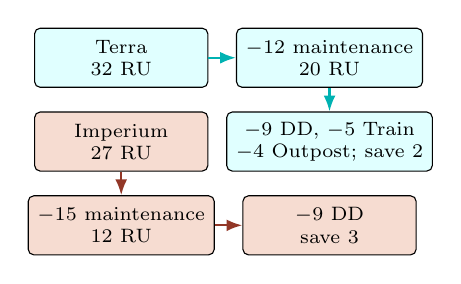
\begin{tikzpicture}[
  box/.style={draw,rounded corners=2pt,align=center,minimum width=2.2cm,
    minimum height=0.75cm,font=\scriptsize},
  arr/.style={-{Latex[length=2mm]},thick}
]
  \node[box,fill=Cyan!12] (ti) {Terra\\32 RU};
  \node[box,fill=Cyan!12,right=0.35cm of ti] (tm) {$-12$ maintenance\\20 RU};
  \node[box,fill=Cyan!12,below=0.3cm of tm] (tb) {$-9$ DD, $-5$ Train\\$-4$ Outpost; save 2};
  \draw[arr,Cyan!70!black] (ti) -- (tm);
  \draw[arr,Cyan!70!black] (tm) -- (tb);

  \node[box,fill=BrickRed!12,below=0.3cm of ti] (ii) {Imperium\\27 RU};
  \node[box,fill=BrickRed!12,below=0.3cm of ii] (im) {$-15$ maintenance\\12 RU};
  \node[box,fill=BrickRed!12,right=0.35cm of im] (ib) {$-9$ DD\\save 3};
  \draw[arr,BrickRed!75!black] (ii) -- (im);
  \draw[arr,BrickRed!75!black] (im) -- (ib);
\end{tikzpicture}
\end{center}

\subsection{C. Terran Player Turn}

\subsubsection{First Movement: the Shuruppak Raid}

The three Beam Scouts at Junction form one stack and jump through Southern
Cross to Sirius. There they split: one Scout stops at Sirius as a reserve while
two continue through Mackhashi and Tau Ceti before entering Shuruppak on their
fifth jump. Each intermediate system is empty. This movement is legal because
a stack composed entirely of Scouts may refuel in any system. An ordinary
mixed fleet would have to stop one jump beyond its last friendly refuelling
site.

Entering Shuruppak reveals the Imperial Mixed Scout and Mixed Destroyer and
ends the two-Scout raiding stack's movement. Space combat is mandatory.

\begin{center}
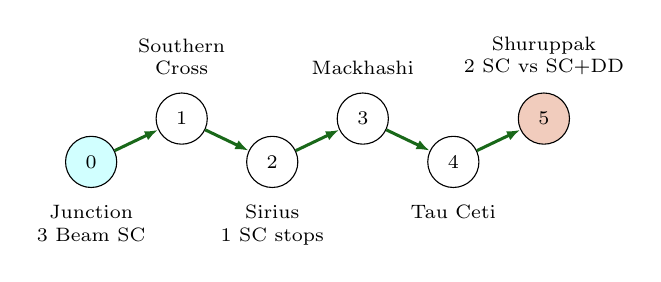
\begin{tikzpicture}[
  sys/.style={circle,draw,minimum size=6.5mm,inner sep=0pt,font=\scriptsize},
  route/.style={draw=ForestGreen!75!black,line width=1.1pt,
    -{Latex[length=1.7mm]}},
  lab/.style={font=\scriptsize,align=center}
]
  \node[sys,fill=Cyan!18] (j) at (0,0) {0};
  \node[sys] (sc) at (1.15,0.55) {1};
  \node[sys] (si) at (2.3,0) {2};
  \node[sys] (ma) at (3.45,0.55) {3};
  \node[sys] (tc) at (4.6,0) {4};
  \node[sys,fill=BrickRed!18] (sh) at (5.75,0.55) {5};
  \draw[route] (j)--(sc);
  \draw[route] (sc)--(si);
  \draw[route] (si)--(ma);
  \draw[route] (ma)--(tc);
  \draw[route] (tc)--(sh);
  \node[lab,below=1mm of j] {Junction\\3 Beam SC};
  \node[lab,above=1mm of sc] {Southern\\Cross};
  \node[lab,below=1mm of si] {Sirius\\1 SC stops};
  \node[lab,above=1mm of ma] {Mackhashi};
  \node[lab,below=1mm of tc] {Tau Ceti};
  \node[lab,above=1mm of sh] {Shuruppak\\2 SC vs SC+DD};
\end{tikzpicture}
\end{center}

The numbered circles show jumps, not movement costs. The route drawing is a
schematic of the printed map rather than a replacement for it.

\subsubsection{First Combat: Round 1 at Long Range}

Terra is the attacker. The initial range is Long. Each side has two ships, so
there is no screening or Fleet Size Bonus.

Before the first firing round, Terra plays \textit{Tactics}, raising its
Tactics from 0 to 1 for this entire battle. Its once-per-round attack reroll is
available, although Terra will not need it in the example.

One Terran Beam Scout performs Point Defense for its group. It forfeits
offensive fire, which costs nothing because Beam ships cannot fire at Long
Range, and the group gains +1 Defense against missiles.

The Imperial Mixed Destroyer has printed Attack 4, reduced to 3 for Mixed
missile fire at Long Range. Against Scout Defense 0 and Point Defense +1, its
Hit Number is $3-0-1=2$; a roll of 4 misses. The Mixed Scout's adjusted Attack
is 2, giving a Hit Number of 1. It rolls a natural 1 and destroys one Hull-1
Terran Scout. Terra removes the non-escort Scout. Its remaining Beam ship has
no legal fire, so the round ends with one Terran ship against two Imperial
ships.

\subsubsection{Round 2: Terra Closes}

Both players select a Scout Picket, worth +2 Maneuver. Terra rolls 7, for
$7+2+1+1=11$; the final +1 is for having the smaller non-Fighter fleet. The
Imperium rolls 4, for $4+2+1=7$. Terra chooses Close Range.

The Imperium now has two ships to one. It screens its Destroyer, forcing the
Terran Scout to target the unscreened Scout. Screening leaves only one
unscreened Imperial ship, however, so the Imperium gives up what would
otherwise have been a $2{:}1$ Fleet Size Bonus.

At Close Range beams fire by class before short-range missiles. The Mixed
Destroyer fires at Class D with adjusted Attack 3 but rolls 6 and misses. At
Class E both sides have Tactics 1, so the Imperial defender fires first. Its
Mixed Scout has adjusted Attack 2 and rolls 5, missing.

The Terran Beam Scout attacks at its full printed Attack 3. The Destroyer is
screened, so it must target the Defense-0 Imperial Scout. It rolls 2 and
destroys that ship with one hit. Because the Imperial Scout chose beam fire,
it could not also make a short-range missile attack had it survived.

\subsubsection{Round 3: Missile Range Restored}

Terra rolls $3+2+1=6$ for Range Control. The surviving Imperial Destroyer uses
its +1 Picket rating and Tactics 1. It rolls $8+1+1=10$ and chooses Long Range.

Neither side can screen or claim Fleet Size. The Terran Scout again performs
Point Defense. The Imperial Destroyer declares High-Intensity Missile Fire:
printed Attack 4, $-1$ for its Mixed Package, and $+1$ for high intensity.
After Point Defense, its Hit Number is $4-0-1=3$. It rolls 2 and destroys the
last raiding Scout before that Scout's Class E opportunity to retreat. The
Imperium retains Shuruppak.

\begin{center}
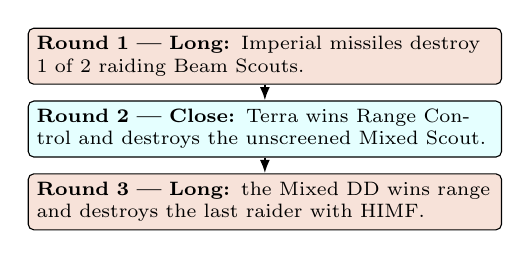
\begin{tikzpicture}[
  rnd/.style={draw,rounded corners=2pt,align=left,text width=5.8cm,
    inner sep=3pt,font=\scriptsize},
  flow/.style={-{Latex[length=1.7mm]},thick}
]
  \node[rnd,fill=BrickRed!10] (r1) {\textbf{Round 1 --- Long:}
    Imperial missiles destroy 1 of 2 raiding Beam Scouts.};
  \node[rnd,fill=Cyan!10,below=2mm of r1] (r2) {\textbf{Round 2 --- Close:}
    Terra wins Range Control and destroys the unscreened Mixed Scout.};
  \node[rnd,fill=BrickRed!10,below=2mm of r2] (r3) {\textbf{Round 3 --- Long:}
    the Mixed DD wins range and destroys the last raider with HIMF.};
  \draw[flow] (r1)--(r2);
  \draw[flow] (r2)--(r3);
\end{tikzpicture}
\end{center}

\subsubsection{Reaction Movement and Combat}

The Imperial player uses the surviving Mixed Destroyer as the one reacting
stack. It jumps from Shuruppak through Tau Ceti and Mackhashi to Sirius, where
it must stop upon encountering the reserve Terran Scout. Three jumps exactly
equal the Imperial Reaction Allowance. The reacting Destroyer is the only
Imperial unit permitted to attack in the Reaction Combat Phase.
Its Missile Depleted marker was removed at the end of the preceding Combat
Phase, so it may make another missile attack in this new phase.

The new battle begins at Long Range. The Terran Scout uses Point Defense; the
Mixed Destroyer's Attack 3 missile therefore has a Hit Number of 2 and its roll
of 7 misses. In round two, Terra rolls $9+2=11$ for Range Control; the Imperium
rolls $4+1+1=6$. Terra chooses Close. The Class D Mixed Destroyer fires first
with adjusted Attack 3, but rolls 8 and misses. At Class E the Terran Beam
Scout rolls a natural 1 and destroys the Hull-1 Destroyer. The attempted
pursuit has cost the Imperium its remaining forward ship.

\subsubsection{Second Movement and Combat}

The surviving reserve Scout returns from Sirius through Southern Cross to
Junction in the Second Movement Phase. Terra has no contested system in its
Second Combat Phase.

The Shuruppak Outpost remains Imperial because no Terran ship remains in orbit.
Even if a Scout had survived, bombardment alone could only remove temporary
Militia; it could not capture the surface. Capturing the Outpost requires a
later fleet with a Transport and surviving troops to pay the occupation cost.

\subsection{D. Imperial Player Turn}

The Imperium uses its two Movement Phases to shift its Carrier, Fighters, and
main surface force toward the Shuruppak corridor. A Fleet Train can move only
one jump in each phase and provides refuelling only when it has not moved in
that particular phase, so the main fleet does not reach Terran space this
turn. Terra declines Reaction Movement. No further combat occurs.

This illustrates why the Scout raid was possible while a combined fleet was
not: self-refuelling is a Scout ability, not a property of every stack that
contains a Scout.

\subsection{E. End Phase}

Temporary combat markers are removed. No World was neutralized and no site
changed ownership, so Glory remains 5. The Terran marker is 1 and the Imperial
marker is 10; neither has reached Glory. Game Turn 2 will begin with the new
Destroyers, Terran Fleet Train, and Terran unplaced Outpost arriving during
Completed Production.

\subsection{Turn 1 Lessons}

\begin{itemize}
  \item Income is collected before maintenance and new production; newly
    purchased units do not appear immediately.
  \item Armament Packages create different preferred ranges without replacing
    the printed \SpaceEmpires\ combat values.
  \item Point Defense can be valuable even when its escort had no legal
    offensive shot.
  \item Range Control can reverse the advantage from round to round.
  \item Reaction Movement creates a real counterstroke, but only reacting
    ships may attack in its Combat Phase.
  \item Space victory and surface conquest are separate achievements.
\end{itemize}

  \clearpage
\section{PLAYER AID}
\small

\subsection{Game Turn}

\begin{tabularx}{\columnwidth}{@{}lX@{}}
\toprule
A & Advance Terran marker up 1; Imperial marker down 1. \\
B & Joint Logistics: politics, connections/income, maintenance, cards,
arrivals, purchases. \\
C & First Player: Move, Combat, enemy Reaction Move/Combat, Move, Combat. \\
D & Second Player repeats the same sequence. \\
E & Clear temporary effects, recover unsupported Worlds, apply delayed Glory,
check victory. \\
\bottomrule
\end{tabularx}

\subsection{Economy and Supply}

\begin{tabularx}{\columnwidth}{@{}Xrr@{}}
\toprule
Income source & Terra & Imperium \\
\midrule
Budget & 0 & 10 \\
Connected World & 8 & 3 \\
Unconnected World & 6 & 1 \\
Connected Outpost & 1 & 0 \\
\bottomrule
\end{tabularx}

Connection paths run through friendly Worlds, Outposts, and Fleet Trains;
enemy combat ships and neutralized sites block them. Ship maintenance equals
Hull Size per ship. Unsupplied ships cost +1 RU and move at most one jump per
Movement/Reaction Phase. Repair at a connected World for 1 RU per hit.

\subsection{Movement}

A normal stack has unlimited jumps but must refuel before leaving each entered
system. Friendly Worlds, Outposts, and stationary Fleet Trains refuel; all-Scout
stacks self-refuel. Enemy combat ships stop movement. Reaction moves one stack
up to the side's allowance (Terra 2, Imperium 3 initially). Fighters need a
base or Carrier; Transports carry six Ground Units.

\subsection{Space Combat}

\begin{tabularx}{\columnwidth}{@{}lXX@{}}
\toprule
Package & Long Range & Close Range \\
\midrule
Beam & --- & Beam full \\
Missile & Missile full & Missile $-1$, after beams \\
Mixed & Missile $-1$ & Beam $-1$ or missile $-2$ \\
\bottomrule
\end{tabularx}

\begin{enumerate}
  \item Reveal groups, packages, and technology. Friendly Bases join.
  \item Round 1 is Long. In later rounds, both sides roll d10 + Picket +
    Tactics; the smaller non-Fighter fleet adds +1. High side chooses range; a
    tie retains it. Then screen; 2:1 unscreened ships earns +1 Attack.
  \item Picket: SC +2, DD +1, CA/CV/TR 0, BC/BB/DN $-1$, none $-2$.
  \item Declare reactions. A Beam/Mixed SC or DD escort forfeits fire to give
    one group +1 Defense vs missiles (+2 at Point Defense 2+). A ship may
    forfeit fire to gain +1 Defense vs beams by dispersing sand.
  \item Long: missiles A--E. Close: beams A--E, then short missiles A--E.
    Higher Tactics wins class ties; defender wins remaining ties.
  \item Hit Number = package-adjusted Attack + Attack Tech + Fleet Bonus
    $-$ Defense $-$ Defense Tech $-$ reactions. Roll d10 at or below; a
    natural 1 always hits. Hull Size hits destroy a ship.
  \item A missile ship may gain +1 Attack, then is Missile Depleted for the
    Combat Phase. At Close Range, an SC, DD, or Fighter may risk defensive
    beam fire to make a +1 Attack Close Assault.
  \item From round 2, a group may retreat instead of firing at its class.
\end{enumerate}

Space Marines may land after space round one; all Ground Units after round two.

\subsection{Planetary Operations}

Outpost/World/Capital generates 1/5/8 Militia. Orbital victor may bombard before
landing; each hit removes one Militia for this Combat Phase only. Permanent
Ground Units give surface Defense 1 (one--three units) or 2 (four or more).

Ground combat uses printed Attack, Defense, Hull, and firing class. Defender
fires first on class ties. No Tactics or Fleet Size. No retreat. Remove one
surviving attacker to occupy: replace a captured Outpost or neutralize a World.
Another Ground Unit or enemy Outpost must remain to hold a neutralized World.

\subsection{Glory Clock}

Imperial capture/loss of an Outpost changes Glory $+1/-1$; neutralizing a World
changes it $+4/-4$. In the End Phase, Terra wins the war if its rising Turn
marker reaches Glory; the Imperium wins if its falling marker reaches Glory.
Capital neutralization wins the campaign immediately.

\subsection{Technology Limits}

In-war research is prohibited. Interwar DP improve Attack, Defense, Tactics,
Fighter, Point Defense, Ground Combat, Capital Construction, or Reaction
Command. Capital Construction 0/1/2/3 allows CA/BC/BB/DN respectively.

\end{document}
